\documentclass{article}
\usepackage[utf8]{inputenc}
\usepackage{mathtools}
\usepackage{titlesec}
\usepackage{indentfirst}
\usepackage{graphicx}
\usepackage{float}


\graphicspath{{PCAPics/}}
\everymath{\displaystyle}
\setcounter{secnumdepth}{4}

\title{Folosirea PCA pentru recunoasterea imaginilor cu ajutorul librariei Accord}
\author{Motrescu Radu}
\date{}

\begin{document}

\maketitle

\newpage

\tableofcontents

\newpage

\section{Libraria Accord.NET}
Libraria Accord.Net contine clase pentru:
\begin{itemize}
\item Calcul stiintific: matematica, statistica si machine learning
\item Procesare de imagini si semnale: imagini, semnale audio si recunoastere si urmarire faciala in timp real
\item Librarii suport pentru controale specifice: histograme, scatter-plots, controale pentru fiecare clasa de procesare imagini si semnale
\end{itemize}


In contextul cerintelor pe care vrem noi sa le indeplinim, vom folosi clase dedicate matematicii, statisticii, si ale unor controale de afisare a datelor. 

\newpage

\section{Ce este PCA?}
PCA, sau Principal Component Analysis, sau pe romaneste, Analiza Componentelor Principale este o unealta matematica aplicata din algebra liniara.

Este o metoda non-parametrica (care nu depinde de statistici) de a extrage informatiile relevante dintr-un set de date complex sau confuz.

\paragraph{Un scurt exemplu: }
Sa presupunem ca am extras informatii pentru 100 de parametri pentru un student: inaltime, varsta, greutate, nota obtinuta la un test, culoarea parului etc. Vrem sa gasim cele mai importante caracteristici care definesc studentul. Cum facem asta? Folosim PCA pentru a selecta numai cele mai importante caracteristici.

\begin{itemize}
	\item Ce parametri dorim sa indepartam:
	\begin{itemize}
	\item Constanti: numarul de capete, care este 1 pentru toti studentii
	\item Aproape constanti: grosimea firului de par: 0.003, 0.002, 0.0005 etc.
	\item Care depind de alti parametri
	\end{itemize}
	\item Ce parametri dorim sa pastram:
	\begin{itemize}
	\item Care nu depind de alti parametri: culoarea ochilor
	\item Care se schimba mult, au variatie mare: notele
	\end{itemize}
\end{itemize}

A putea elimina parametrii irelevanti si a-i pastra pe cei relevanti este usor pentru un om, el putand vedea clar care parametri nu exprima informatii relevante despre subiectul respectiv, dar cum putem face calculatorul sa isi dea seama de acesti parametri? Folosind matematica, desigur!

Dorim sa minimizam "sunetul de fundal" si redundanta datelor si sa maximizam variatia dintre parametri.

Se poate vedea in imaginea de mai jos maximizarea variatiei dintre axele norului de puncte respectiv.

\begin{figure}[H]
\centering
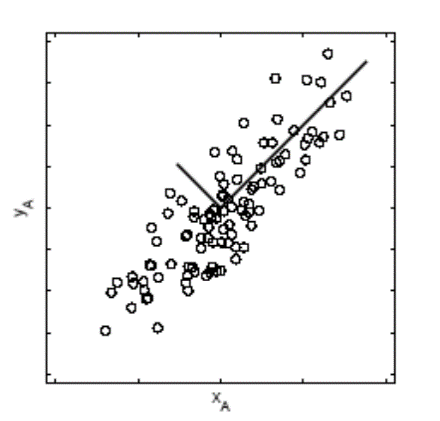
\includegraphics[scale=0.5]{Picture1}
\end{figure}

In imaginile de mai jos se pot vedea inregistrarile unor informatii. In imaginea (a) si (b) se poate vedea cum informatiile nu sunt corelate, avand redunanta mica spre medie (ex: inaltimea unui student si media lui), iar in imaginea (c) se poate vedea o redundanta mare, insemnand ca ambii parametrii pot fi exprimati unul in functie de celalalt.

\begin{figure}[H]
\centering
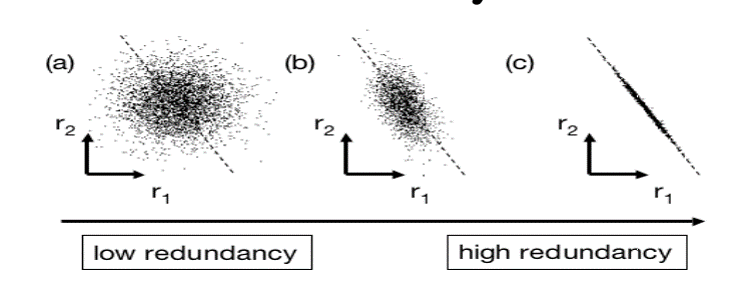
\includegraphics[width=\linewidth]{Picture2}
\end{figure}

\paragraph{Variatia} Este un mijloc de realizare a variabilitatii datelor dintr-un set de date cu media $\overline{X}$:

\begin{equation}
\sigma^2=\frac{\sum_{i=1}^{n} \left( X_i - \overline{X} \right)^2 }{n-1}
\end{equation}

\paragraph{Covariatia} Reprezinta variabilitatea fiecarei dimensiuni in relatie cu celelalte, si este masurata intre 2 dimensiuni pentru a se putea observa relatia dintre cele 2, spre exemplu numarul de ore studiate si nota obtinuta la examen.

\begin{equation}
\text {var} \left( X \right) = \frac{\sum_{i=1}^{n} \left( X_i - \overline{X} \right) \left( X_i - \overline{X} \right) }{n-1}
\end{equation}


\begin{equation}
\text {cov} \left( X,Y \right) = \frac{\sum_{i=1}^{n} \left( X_i - \overline{X} \right) \left( Y_i - \overline{Y} \right) }{n-1}
\end{equation}


\paragraph{Matricea de covariatie}
Consideram setul de date din care extragem valoarea medie (zero-mean data) si avand setul de vectori \( \left\{ x_1, x_2, ..., x_m \right\} \) care reprezinta liniile unei matrici $X_{m,n}$.

Fiecare linie a matricii reprezinta toate masuratorile unui anumit parametru, iar fiecare coloana reprezinta masuratorile care s-au intamplat la un moment dat.

De aici ajungem la definitia matricei de covariatie:

\begin{equation}
S_x \equiv \frac{1}{n-1}XX^T \text { where } X = 
\begin{bmatrix}
x_1 \\ \vdots \\ x_m
\end{bmatrix}
\end{equation}

$S_x$ este o matrice simetrica $m \times m$, termenii de pe diagonala reprezentand variatia din acelasi parametru, iar termenii care nu sunt de pe diagonala reprezinta covariatia dintre parametri diferiti. Calculand $S_x$, cuantificam corelatia dintre toate posibilele perechi de masuratori. Observand elementele din matrice, o cavariatie mare reprezinta un caz de redundanta mare, iar o covariatie egala cu 0 reprezinta date complet necorelate.

\begin{equation}
C=\begin{bmatrix}
cov(X,X) && cov(X,Y) && cov(X,Z) \\
cov(Y,X) && cov(Y,Y) && cov(Y,Z) \\
cov(Z,X) && cov(Z,Y) && cov(Z,Z)
\end{bmatrix}
\end{equation}


\paragraph{Valorile si vectorii proprii}
Urmatorul pas in calcularea PCA este aflarea valorilor si a vectorilor proprii ale matricii de covariatie. Extragand aceste informatii, ele ne vor arata componentele principale ale setului de date: vectorul propriu cu cea mai mare valoare proprie este componenta principala a setului de date. Se obisnuieste sortarea vectorilor proprii in functie de valoarea proprie pentru a determina ordinea de semnificativitate.

Vectorii si valorile proprii reies din probleme de urmatoarea forma:
\begin{equation}
A.v= \lambda . v
\end{equation}

\textbf{A}: matrice $m \times m$


\textbf{v}: vector $m \times 1$  nenul


$\lambda$: constanta

Pentru orice valoare a lui $\lambda$ pentru care ecuatia are solutie se numeste valoarea proprie a lui A, si vectorul \textbf{v} care corespunde acestei valori se numeste vectorul propriu a lui A.

\paragraph{Pasul final PCA} este sa aflam valorile finale ale setului de date. Aici avem optiunea sa ignoram o parte din dimensiunile pe care le avem, deoarece ele pot fi nesemnificative, avand valori proprii mici, sau dorim afisarea lor in 1, 2 sau 3 dimensiuni. Dupa stabilirea vectorilor proprii doriti, aflarea datelor finale este simpla, proiectam punctele in spatiul lor: 

FinalData = RowFeatureVector $\times$ RowZeroMeanData

\textbf{RowFeatureVectore} este matricea cu vectorii proprii transpusi, cu cel mai semnificati vector propriu pe prima linie.

\textbf{RowZeroMeanData} este matricea care contine setul de date initial din care s-a scazut valorea medie.

Matricea rezultata \textbf{FinalData} va contine setul de date dupa aplicarea algoritmului PCA.
\newpage

\section{Jurnalul dezvoltarii aplicatiei}

\end{document}
